\section{Propuesta}

\subsection{Conjunto de datos a utilizar}

Para realizar este trabajo utilizaremos un conjunto de datos con $960$ muestras de la sínfisis púbica clasificados manualmente por investigadores del Laboratorio de Antropología Física de la Universidad de Granada utilizando las diez fases propuestas por Todd.

Este conjunto de datos se divide en dos partes, las muestras tomadas de la lateralidad izquierda ($473$ muestras) y la lateralidad derecha ($487$ muestras) del pubis.

\subsubsection{Problema del balanceo de clases}

Como vimos en la figura \ref{fig:conteo_original} con el conteo de cada una de las fases en el conjunto completo, los datos de este problema se encuentran altamente desbalanceados, hay rangos de edades en las que apenas contamos con datos, y la diferencia entre número de datos entre una edad temprana y alta es muy grande. De cara a resolver este problema proponemos utilizar un algoritmo de sobremuestreo de datos, al igual que en \cite{NSLVOrdAge}.

En este artículo se proponen distintas técnicas de sobremuestreo, principalmente utilizando un sobremuestreo de forma aleatoria, utilizando el algoritmo SMOTE \cite{revisionSMOTE} (y varias variaciones de este algoritmo) y el algoritmo ADASYN \cite{propuestaADASYN}.

En nuestro caso, al utilizar el mismo conjunto de datos, podemos ver en su artículo que la técnica que mejor ha funcionado para este conjunto de datos es Borderline-SMOTE, así que también utilizaremos esta técnica aunque tendremos en cuenta otras para comprobar si con nuestro enfoque otras técnicas permiten mejorar los resultados del modelo.

\subsubsection{Enfoque con el que trabajaremos el conjunto de datos}


\begin{figure}[H]
    \centering
	  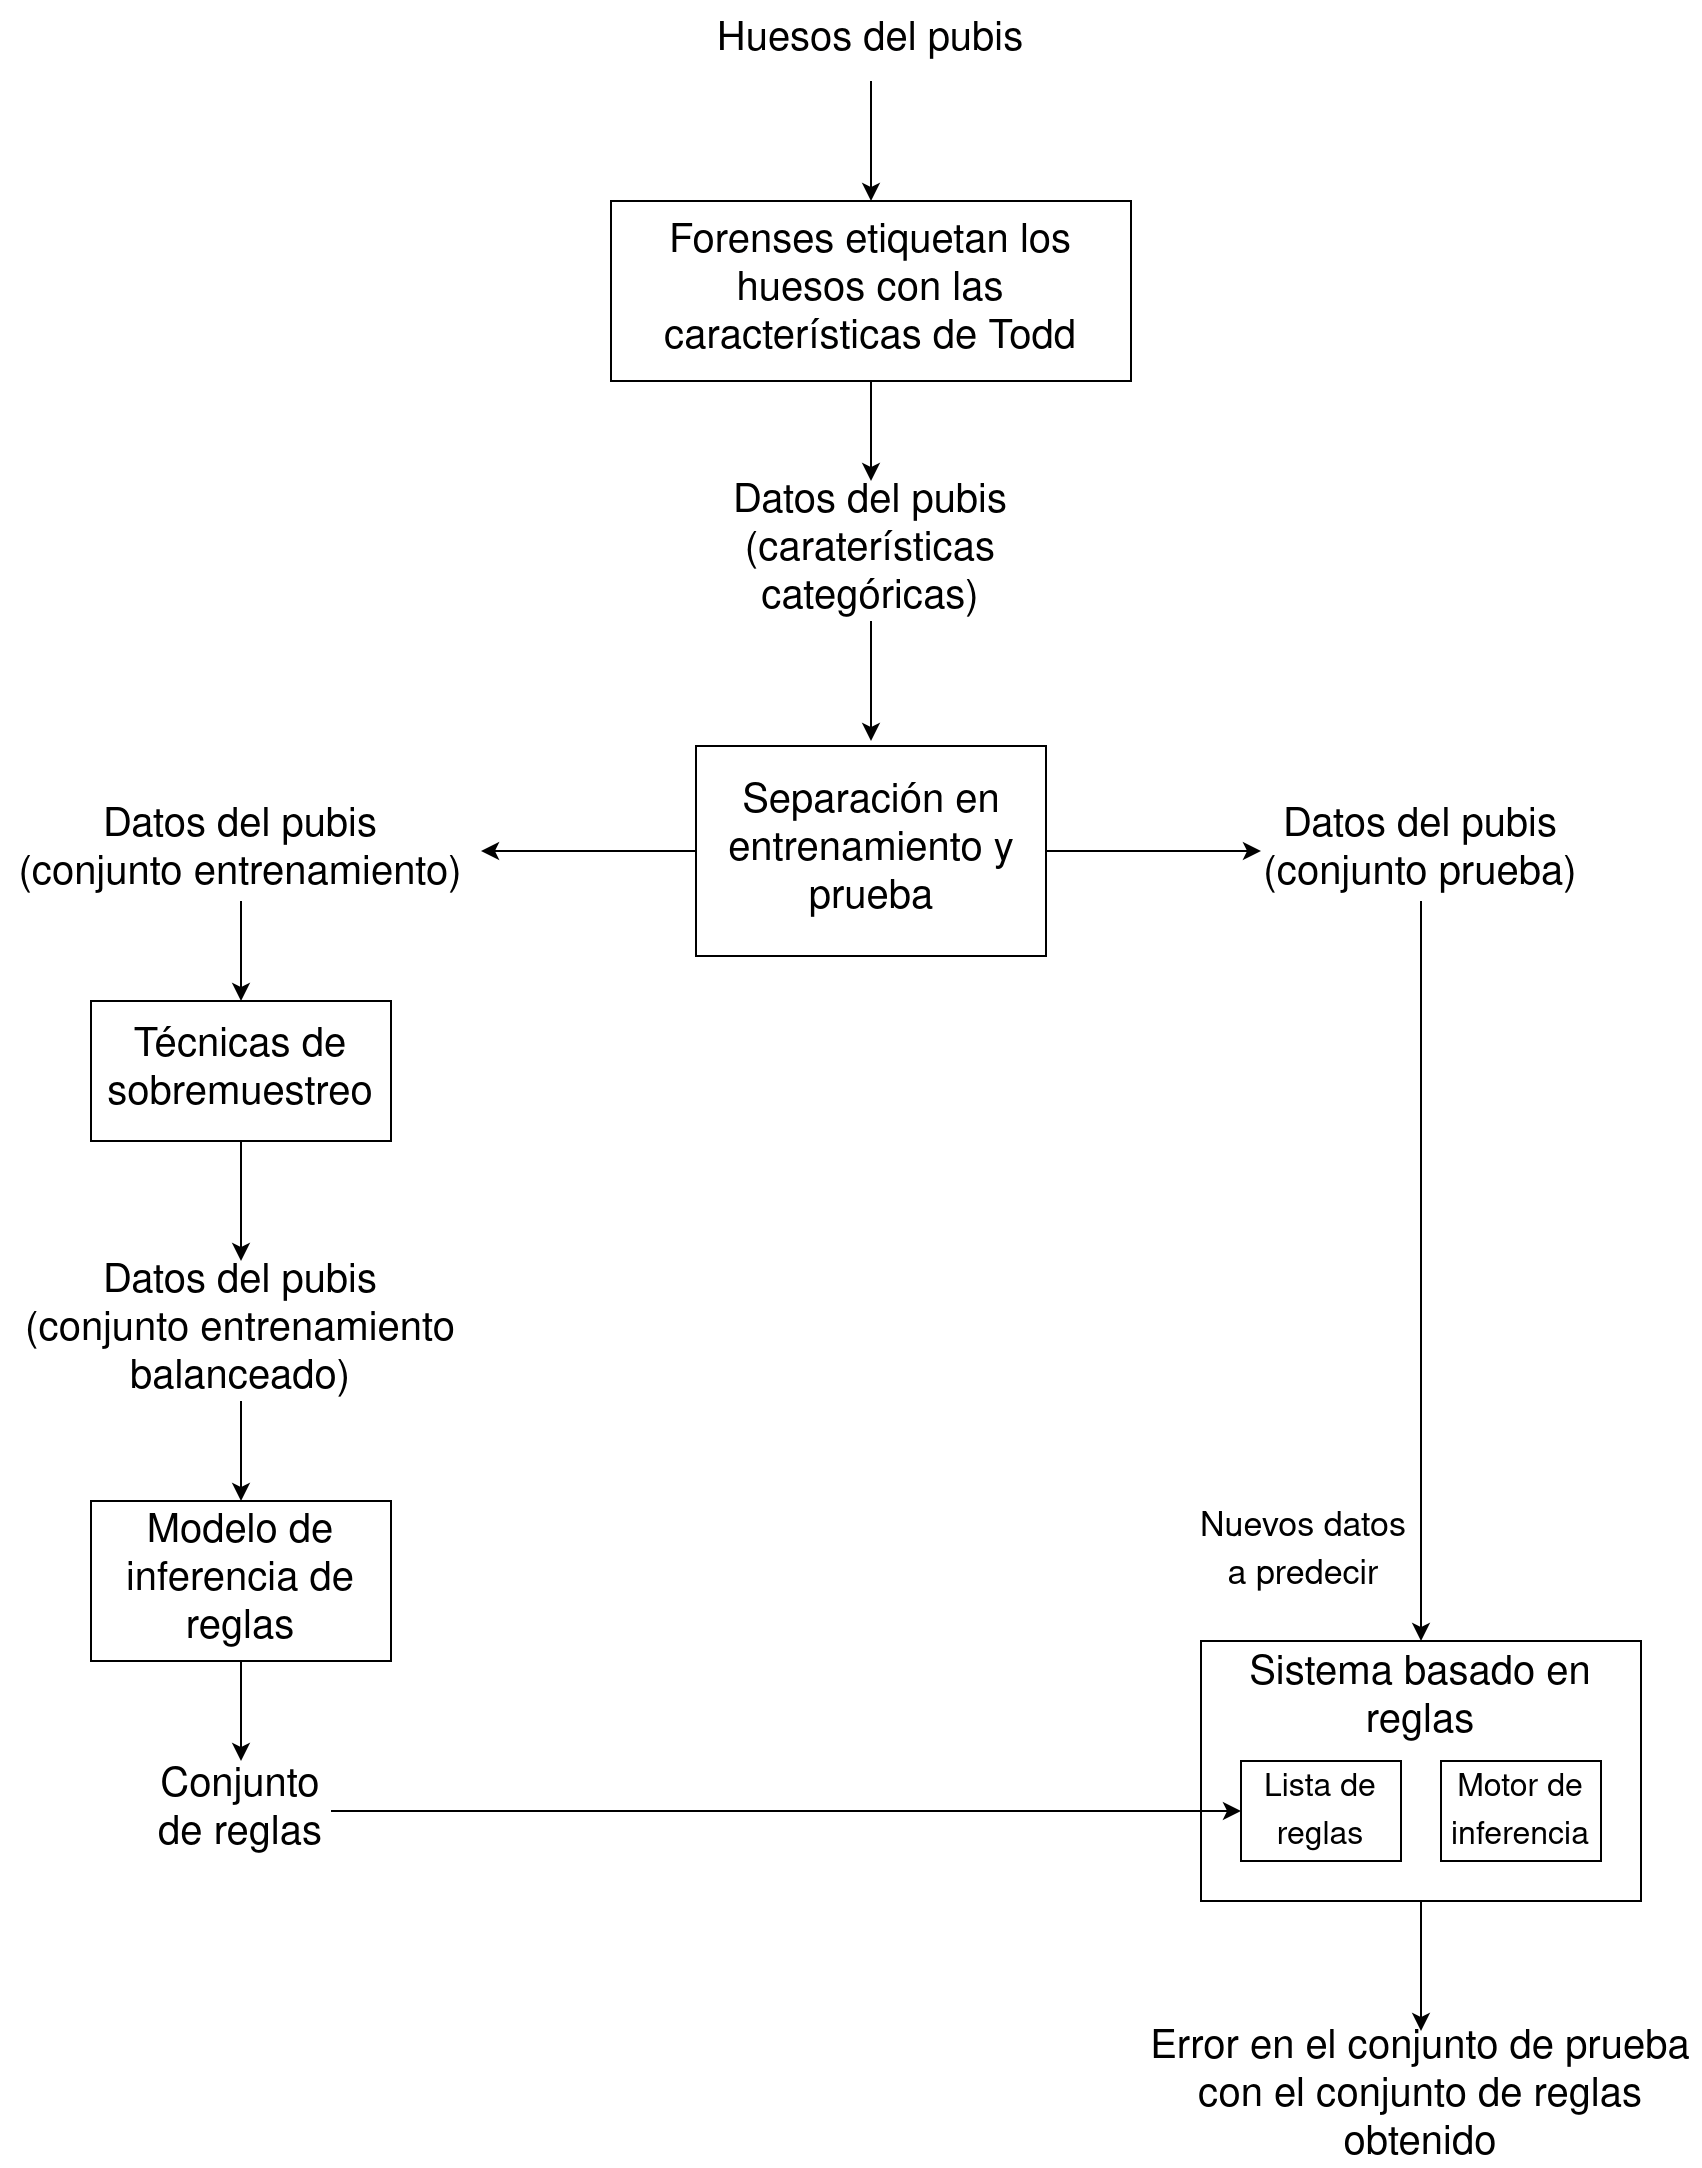
\includegraphics[width=0.8\textwidth]{esquema_datos.png}
    \caption{Esquema general de los pasos que seguirá el conjunto de datos para entrenar y validar el modelo.}
	 \label{fig:esquema_datos}
\end{figure}

En la figura \ref{fig:esquema_datos} podemos ver el flujo que seguirán los datos de entrada, a falta de concretar el sistema de validación a utilizar, validación cruzada, que se explicará más adelante.

\newpage

\subsection{Algoritmos a utilizar y experimentación}

De cara a la experimentación se propone utilizar \textit{R} para realizar el análisis de los datos debido a la gran cantidad de bibliotecas y herramientas que ofrece, mientras que se utilizará \textit{Python} para aplicar parte del preprocesado de los datos ya que este lenguaje cuenta con múltiples herramientas para análisis de datos así como muchos de los métodos que vamos a utilizar.

Para los algoritmos de aprendizaje utilizados, que se describirán más adelante, se utilizará JCLEC, un software desarrollado en Java para computación evolutiva, que al ser software libre podremos modificar para nuestras necesidades.


% TODO plantear ir añadiendo una planificación temporal

% \subsection{Planificación temporal}

\newpage
